% arara: lualatex
% arara: bibtex
% arara: lualatex
% arara: lualatex
\PassOptionsToPackage{dvipsnames}{xcolor}
\documentclass{beamer}
\usetheme{metropolis}           % Use metropolis theme
\usepackage{xcolor}
\usepackage{graphicx}
\usepackage{lstautogobble}
\newcommand{\issuelink}{https://github.com/GrammaticalFramework/GF/issues/5}
\newcommand{\PRlink}{https://github.com/GrammaticalFramework/GF/pull/9}

\newcommand{\translation}[1]{{\tiny\texttt{#1}}}

\usepackage{listings}
\lstset{
  autogobble=true,
  breaklines=true,
  language=ML,
  showstringspaces=false,
  basicstyle=\tiny\ttfamily,
  keywordstyle=\bfseries\color{Bittersweet!40!black},
  commentstyle=\itshape\color{Violet!40!black},
  identifierstyle=\color{BurntOrange},
  stringstyle=\color{RoyalBlue},
  inputencoding=utf8,
  escapeinside={\%*}{*)},
  literate={ç}{{\color{BurntOrange}\c{c}}}1 {ş}{{\c{s}}}1
  %% {ğ}{{\u{g}}}1
  %% {Ğ}{{\u{G}}}1
  %% {ı}{{\i}}1
    %% {İ}{{\.{I}}}1
    %% {ö}{{\"o}}1
    %% {Ö}{{\"O}}1
    %% {Ş}{{\c{S}}}1
    %% {ü}{{\"u}}1
    %% {Ü}{{\"U}}1
}

\usepackage{hyperref}
\hypersetup{
  colorlinks=true,
  linkcolor=Bittersweet,
  citecolor=RoyalBlue,
}
\title{Reviving the Turkish resource grammar}
\date{\today}
\author{Ayberk Tosun}
\institute{Fifth GF Summer School}
\begin{document}
  \maketitle

  \section{Overview}

  \begin{frame}{Introduction}
    \begin{itemize}
      \item<1-> Some non-trivial work was done\footnote{Thanks to Server
        \c{C}imen and Krasimir Angelov} on the Turkish resource grammar (RG).
        \begin{itemize}
          \item<2-> Nevertheless, the Turkish RG is of no use
            because of the missing functionality.
        \end{itemize}
      \item<3-> This work was done a long time ago (about $8$ years).
      \item<4-> \emph{Short story}: the Turkish RG won't complete
        itself; someone has to do some work.
    \end{itemize}
  \end{frame}

  \begin{frame}{What's missing?}
    \begin{itemize}
      \item<1-> According to \texttt{pg -missing} the linearizations of around
        $470$ functions are missing
      \item<2-> The relevant issue on GitHub: \href{\issuelink}{\alert{\#5}}.
    \end{itemize}
  \end{frame}

  \section{\texttt{StructuralTur.gf}}

  \begin{frame}{New linearizations in \texttt{StructuralTur.gf}}
    \scriptsize
    \begin{itemize}
      \item \texttt{with\_Prep}
      \item \texttt{before\_Prep}
      \item \texttt{above\_Prep}
      \item \texttt{behind\_Prep}
      \item \texttt{on\_Prep}
      \item \texttt{in\_Prep}
      \item \texttt{except\_Prep}
      \item \texttt{during\_Prep}
      \item \texttt{between\_Prep}
      \item \texttt{and\_Conj}
      \item \texttt{or\_Conj}
      \item \texttt{always\_Adv}
      \item \texttt{but\_PConj}
      \item \texttt{everybody\_NP}
      \item \texttt{everything\_NP}
      \item \texttt{many\_Det}
    \end{itemize}
    \normalsize
  \end{frame}

  \begin{frame}[fragile]{Testing \texttt{StructuralTur.gf} out}
    \begin{itemize}
      \item<1->
        \begin{lstlisting}
        Lang> parse -lang=LangEng -cat=Cl "everybody always eats everything"
        \end{lstlisting}
      \item<2->
        \begin{lstlisting}
         --> PredVP everybody_NP
               (AdVVP always_AdV
                 (ComplSlash (SlashV2a eat_V2) everything_NP))
        \end{lstlisting}
      \item<3->
        \begin{lstlisting}
        Lang> parse -lang=LangEng -cat=Cl "everybody always eats everything"
                | l -lang=LangTur
        \end{lstlisting}
      \item<4->
        \begin{lstlisting}
        --> %*herkes her zaman herşeyi yiyor*)
        \end{lstlisting}
      \item<5->
        \begin{lstlisting}
          Lang> parse -lang=LangEng -cat=Cl "everybody always eats many apples"
                  | l -lang=LangTur
        \end{lstlisting}
      \item<6->
        \begin{lstlisting}
          --> %*herkes her zaman birçok elmayı yiyor*)
        \end{lstlisting}
    \end{itemize}
  \end{frame}

  \section{\texttt{AdjectiveTur.gf}}

  \begin{frame}{Progress on \texttt{AdjectiveTur.gf}}
    \begin{itemize}
      \item<1-> The \texttt{AdjectiveTur} module didn't exist before.
      \item<2-> Now it contains the implementations for the following:
        \begin{itemize}
          \item \texttt{ComparA}
          \item \texttt{UseComparA}
          \item \texttt{AdvAP}
          \item \texttt{AdAP}
          \item \texttt{UseA2}
          \item \texttt{ComplA2}
          \item \texttt{ReflA2}
        \end{itemize}
    \end{itemize}
  \end{frame}

  \begin{frame}[fragile]{Playing with \texttt{AdjectiveTur.gf}}
    \begin{itemize}
      \item<1->
        \begin{lstlisting}
          Lang> l -lang=LangEng ReflA2 married_A2
        \end{lstlisting}
      \item<2->
        \begin{lstlisting}
          --> %*married to myself*)
        \end{lstlisting}
      \item<3->
        \begin{lstlisting}
          Lang> l -lang=LangTur ReflA2 married_A2
        \end{lstlisting}
      \item<4->
        \begin{lstlisting}
          --> %*kendi ile evli*)
        \end{lstlisting}
    \end{itemize}
  \end{frame}

  \section{\texttt{NounTur.gf}}

  \begin{frame}{Progress on \texttt{NounTur.gf}}
    \begin{itemize}
      \item \texttt{MassNP}
      \item \texttt{ComplN2}
      \item \texttt{AdjCN}
      \item \texttt{AdvCN}
      \item \texttt{AdvNP}
    \end{itemize}
  \end{frame}

  \begin{frame}[fragile]{Testing \texttt{NounTur.gf} out}
    \begin{itemize}
      \item<1->
        \begin{lstlisting}
          Lang> parse -cat=CN -lang=LangEng "beer worse than everything"
        \end{lstlisting}
      \item<2->
        \begin{lstlisting}
          --> AdjCN (ComparA bad_A everything_NP) (UseN beer_N)
        \end{lstlisting}
      \item<3->
        \begin{lstlisting}
          Lang> parse -cat=CN -lang=LangEng "beer worse than everything"
                  | l -lang=LangTur
        \end{lstlisting}
      \item<4->
        \begin{lstlisting}
          %*--> herşeyden kötü bira*)
        \end{lstlisting}
    \end{itemize}
  \end{frame}

  \section{Some challenges}

  \begin{frame}{Finding problems or \emph{monsters}}
    \begin{itemize}
      \item<1-> Programs are developed through series of assertions---those
        of \emph{correctness}.
      \item<2-> Of course, these assertions do not always hold; one soon finds a
        nasty counterexample (monster\footnote{See ``Proofs and Refutations''
        by Lakatos (\cite{lakatos1976proofs})}).
          \begin{itemize}
            \item<3-> Usually \alert{proof-directed debugging} is a good way
              \cite{harper1999proof}.
          \end{itemize}
      \item<4-> How one will avoid this monster determines the further
        development of the program.
      \item<5-> \emph{The problem}: how do you find such monsters for a resource
        grammar?
    \end{itemize}
  \end{frame}

  \begin{frame}{Do I know Turkish, even?}
    \begin{itemize}
      \item<1-> ``kendi'' is simply the reflexive pronoun in Turkish.
        \begin{itemize}
          \item<2-> \dots or so did I think
        \end{itemize}
      \item<3-> Then I decided to consult the standard Turkish grammar
        textbook \cite{goksel2004turkish}.
      \item<4->
        \begin{center}
          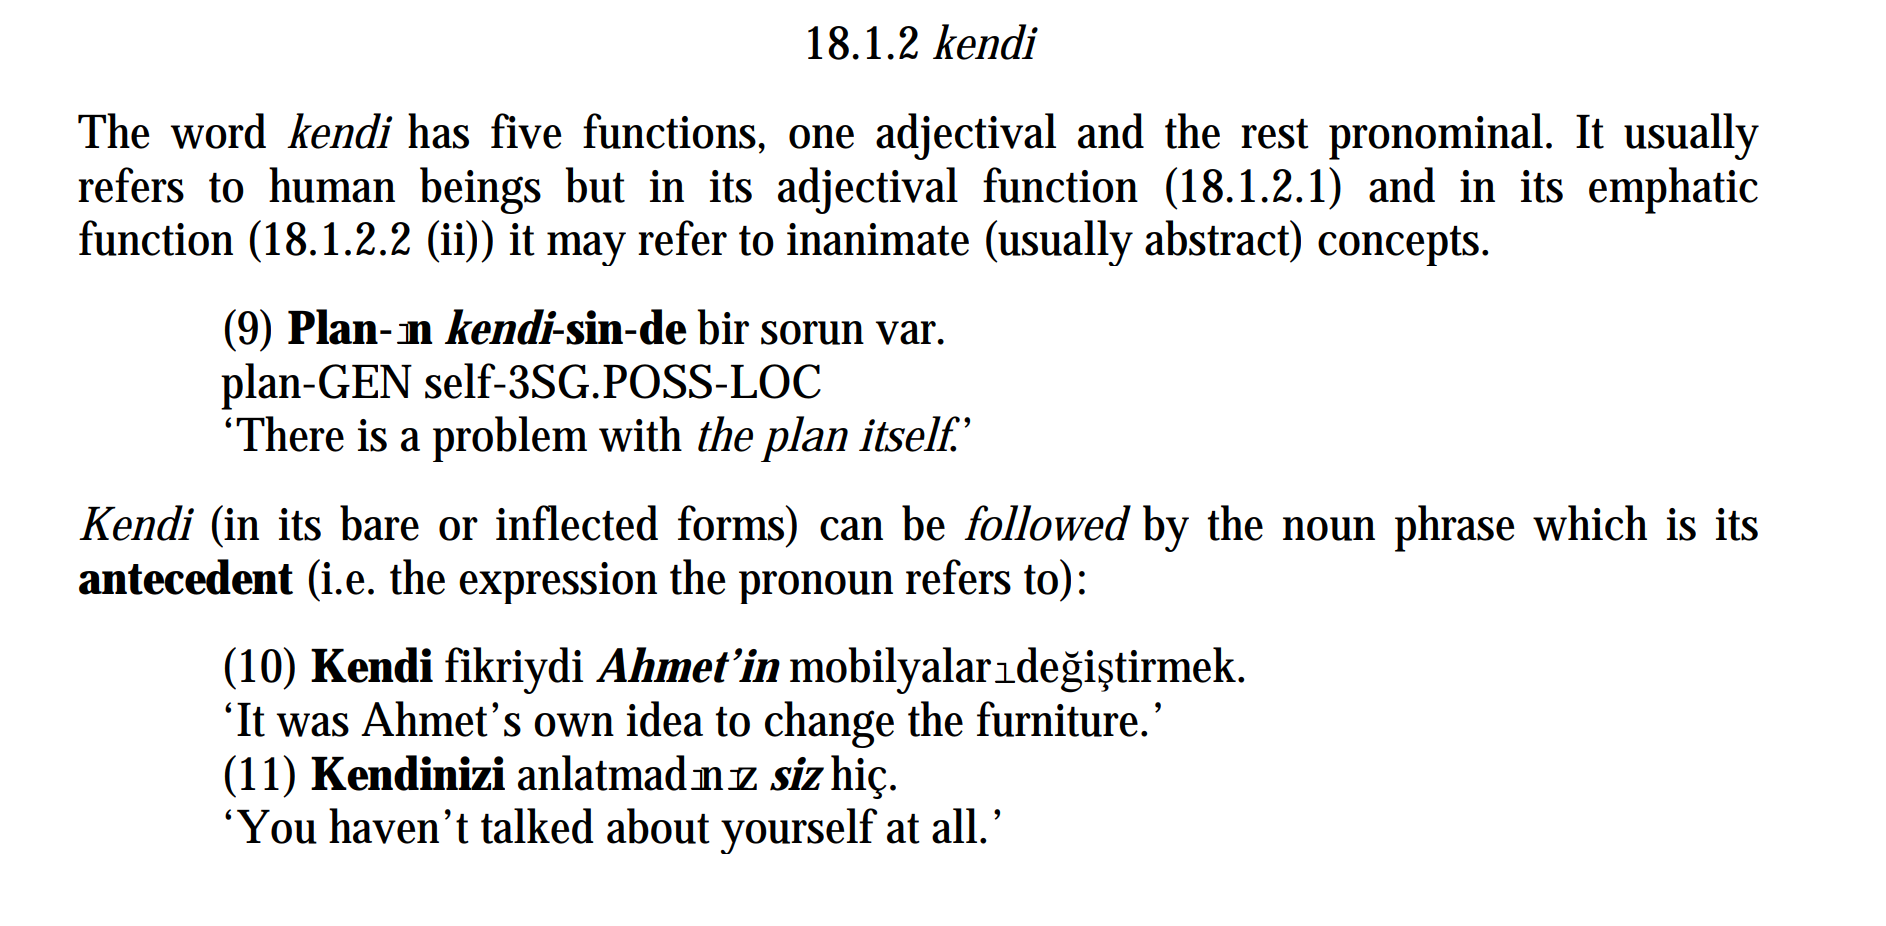
\includegraphics[scale=0.3]{resources/kendi-functions.png}
         \end{center}
    \end{itemize}
  \end{frame}

  \begin{frame}{Do I know Turkish, even?}
    \begin{itemize}
      \item<1-> 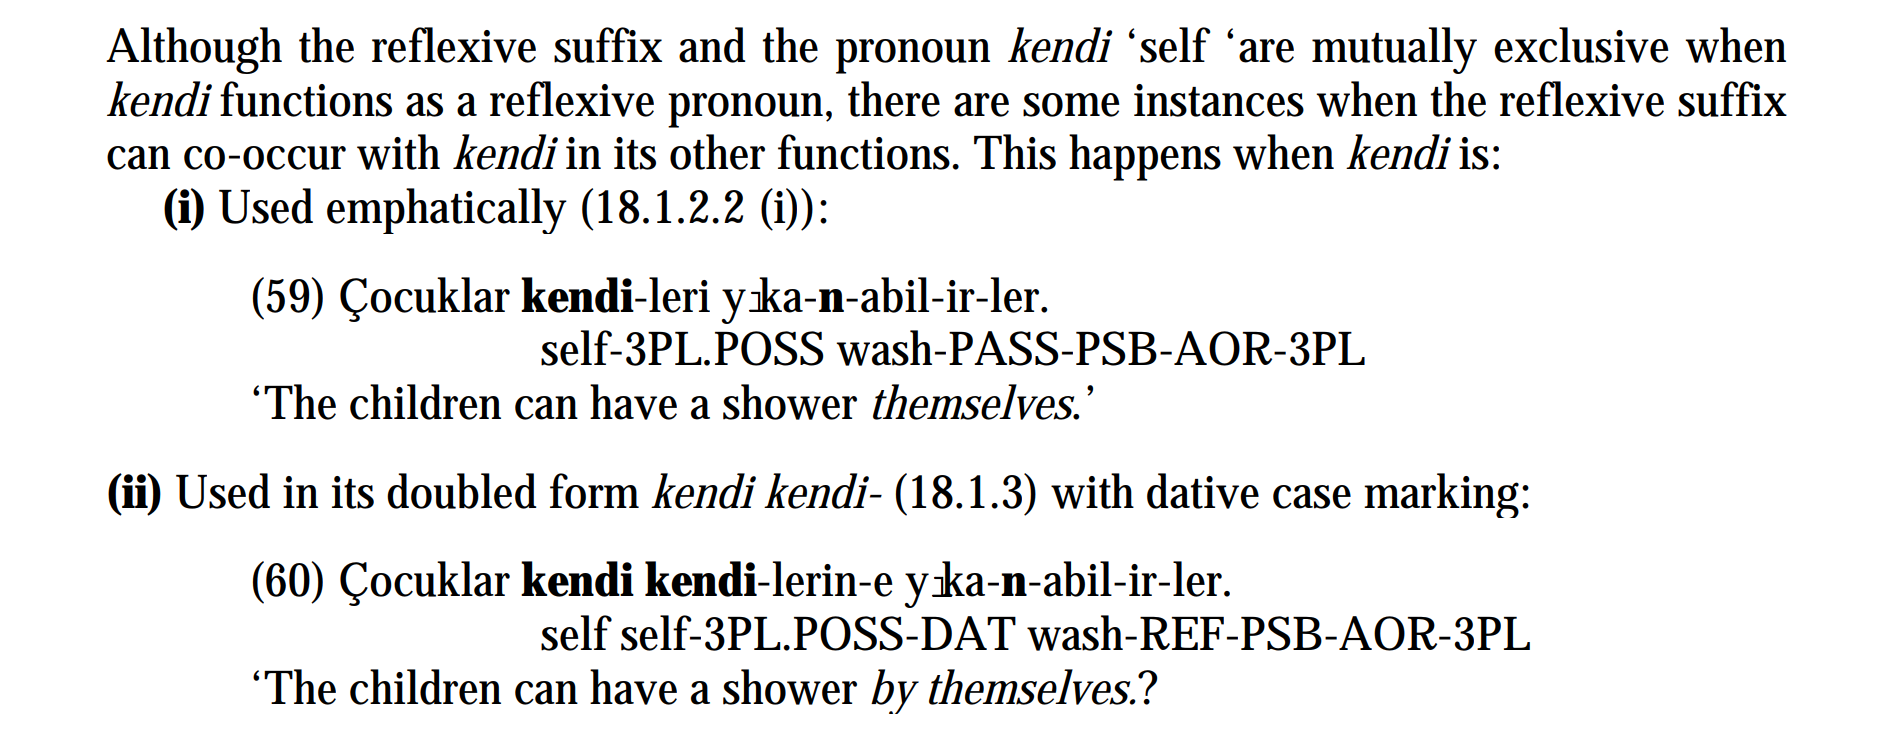
\includegraphics[scale=0.35]{resources/kendi-exceptions.png}
      \item<2-> Some of these take a non-trivial queryign of one's native
        speaker intuitions.
    \begin{itemize}
  \end{frame}

  \section{Concluding Remarks}

  \begin{frame}{The future}
    \begin{itemize}
      \item<1-> Current status: first PR merged into \texttt{GF/master}.
      \item<2-> Continuing work on my fork of GF, branches:
        \begin{itemize}
          \item<2-> \texttt{ayberkt/GF:structural}
          \item<2-> \texttt{ayberkt/GF:adjectives}
        \end{itemize}
      \item<3-> Hopefully, I will keep working through the semester.
      \item<4-> The goal is to get Turkish into the offline translation tool.
    \end{itemize}
  \end{frame}

  \begin{frame}{Acknowledgments}
    \Large
      Thanks to \emph{Krasimir Angelov} for all his help.
  \end{frame}

  \begin{frame}{Goodbye!}
    \begin{itemize}
    \item<1-> \alert{It was very nice meeting you all!}
    \item<2-> Stay in touch:
      \begin{itemize}
        \item<3-> I am \alert{\texttt{ayberkt}} everywhere on the internet.
        \item<4-> You can mail me at \texttt{ayberk.tosun@gmail.com}.
      \end{itemize}
    \end{itemize}
  \end{frame}

  \bibliographystyle{alpha}
  \bibliography{bibliography}

\end{document}
